\cp{\section{Design Challenges of \pname{}}}
\label{motiv}

\begin{figure}
	\centering
	\subfigure[Recall Ratio]{
		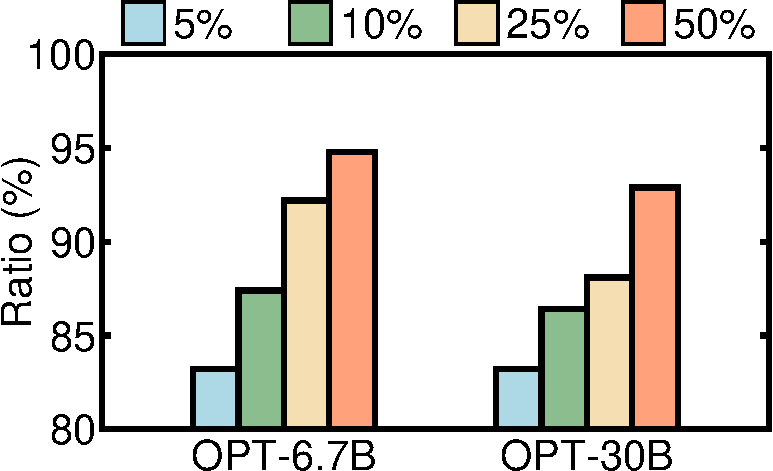
\includegraphics[width=1.5in, height=1in]{static_recall.pdf}
		\label{fig:static-recall}
	}
	\hspace{0.06in}
	\subfigure[Generation Quality]{
		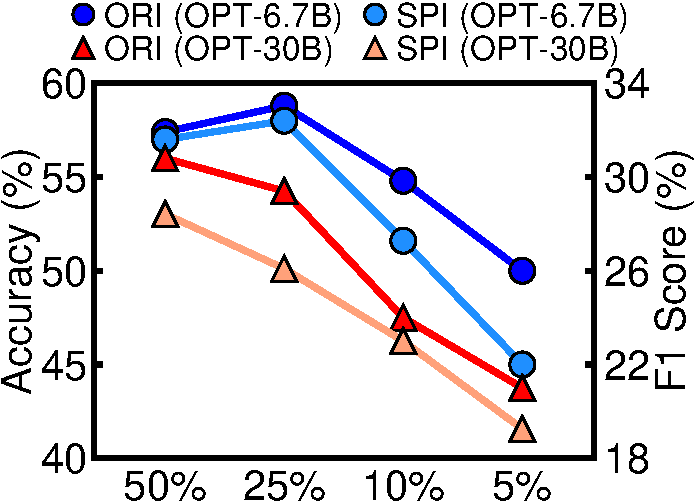
\includegraphics[width=1.5in, height=1in]{static_acc.pdf}
		\label{fig:static-acc}
	}
	\caption{The recall ratios and the impacts on model generation quality of the static pre-identification method (SPI) under various important token retention percentages. `ORI' denotes the baseline where the SPI method is not applied.}
	\label{fig:static_methods}
\end{figure}


\noindent \textbf{Challenge 1: Importance identification introduces high I/O overhead for prefix KV loading.}
\cp{Existing methods identify important KVs by loading all prefix keys (K) into GPU memory~\cite{h2o-nips23, infinigen-osdi24, flexgen-icml23, scissorhands-nips23}, 
so reducing only the loading time of values (V) yields limited TTFT gains. 
A naive solution to reduce I/O overhead is to pre-record the important tokens of each prefix based on prior queries and load only their KVs when the same prefix reappears. 
However, this static approach fails to account for query-dependent token importance. 
In practice, token relevance within the same prefix can vary significantly across different queries. 
In RAG, for example, different queries sharing the same document prefix may attend to different segments, 
causing static selection to miss critical tokens and degrade accuracy. 
We evaluate this limitation using OPT-6.7B on RTE~\cite{lmeval} and OPT-30B on SQuAD~\cite{squad-arxiv18}, 
measuring accuracy and F1 score~\cite{cachegen-sigcomm24}, respectively. 
As shown in Figure~\ref{fig:static_methods}, even with recall ratios above 80\%, 
missing key KVs reduces accuracy by up to 5\% on RTE and 3.3\% on SQuAD. 
These results motivate a dynamic approach that identifies important tokens per query while minimizing I/O overhead.}





%Existing methods must load all prefix keys into GPU
%memory to compute attention weights and then identify important
%KVs~\cite{h2o-nips23, infinigen-osdi24, flexgen-icml23,
%	scissorhands-nips23}. 
%Reducing only the loading time of prefix values limits TTFT reduction.
%
%A straightforward approach to avoid loading all prefix keys is to statically record the identified important tokens for queries. Then, when another query with the same prefix arrives, only the KVs of pre-identified important tokens would be loaded, reducing the I/O time.
%However, this approach has a significant flaw. We observed that the importance
%of tokens within the same prefix can vary depending on the specific query. We
%intuitively explain the observation here. For example, in a RAG scenario,
%different queries might use the same document as the prefix, but the relevant
%answers could be found in different text segments of the prefix. 
%Thus, the method that pre-identifies important tokens could miss critical ones, substantially degrading the accuracy of LLM inference.

% To validate this flaw, we test the important token recall ratio and its impact on model generation quality using two models and two datasets: OPT-6.7B on the RTE~\cite{lmeval} dataset and OPT-30B on the SQuAD~\cite{squad-arxiv18} dataset. We measure model generation quality using accuracy and F1 score, on these two datasets respectively. Figure~\ref{fig:static_methods} shows that although the recall rate exceeds 80\%, missing important KVs led to a drop in accuracy and F1 score of up to 5\% on the RTE dataset and 3.3\% on the SQuAD dataset.
% Hence, an intelligent method is required that can dynamically identify important tokens within a prefix for different queries while introducing minimal I/O overhead.




\begin{figure}
	\centering
	\subfigure[]{
		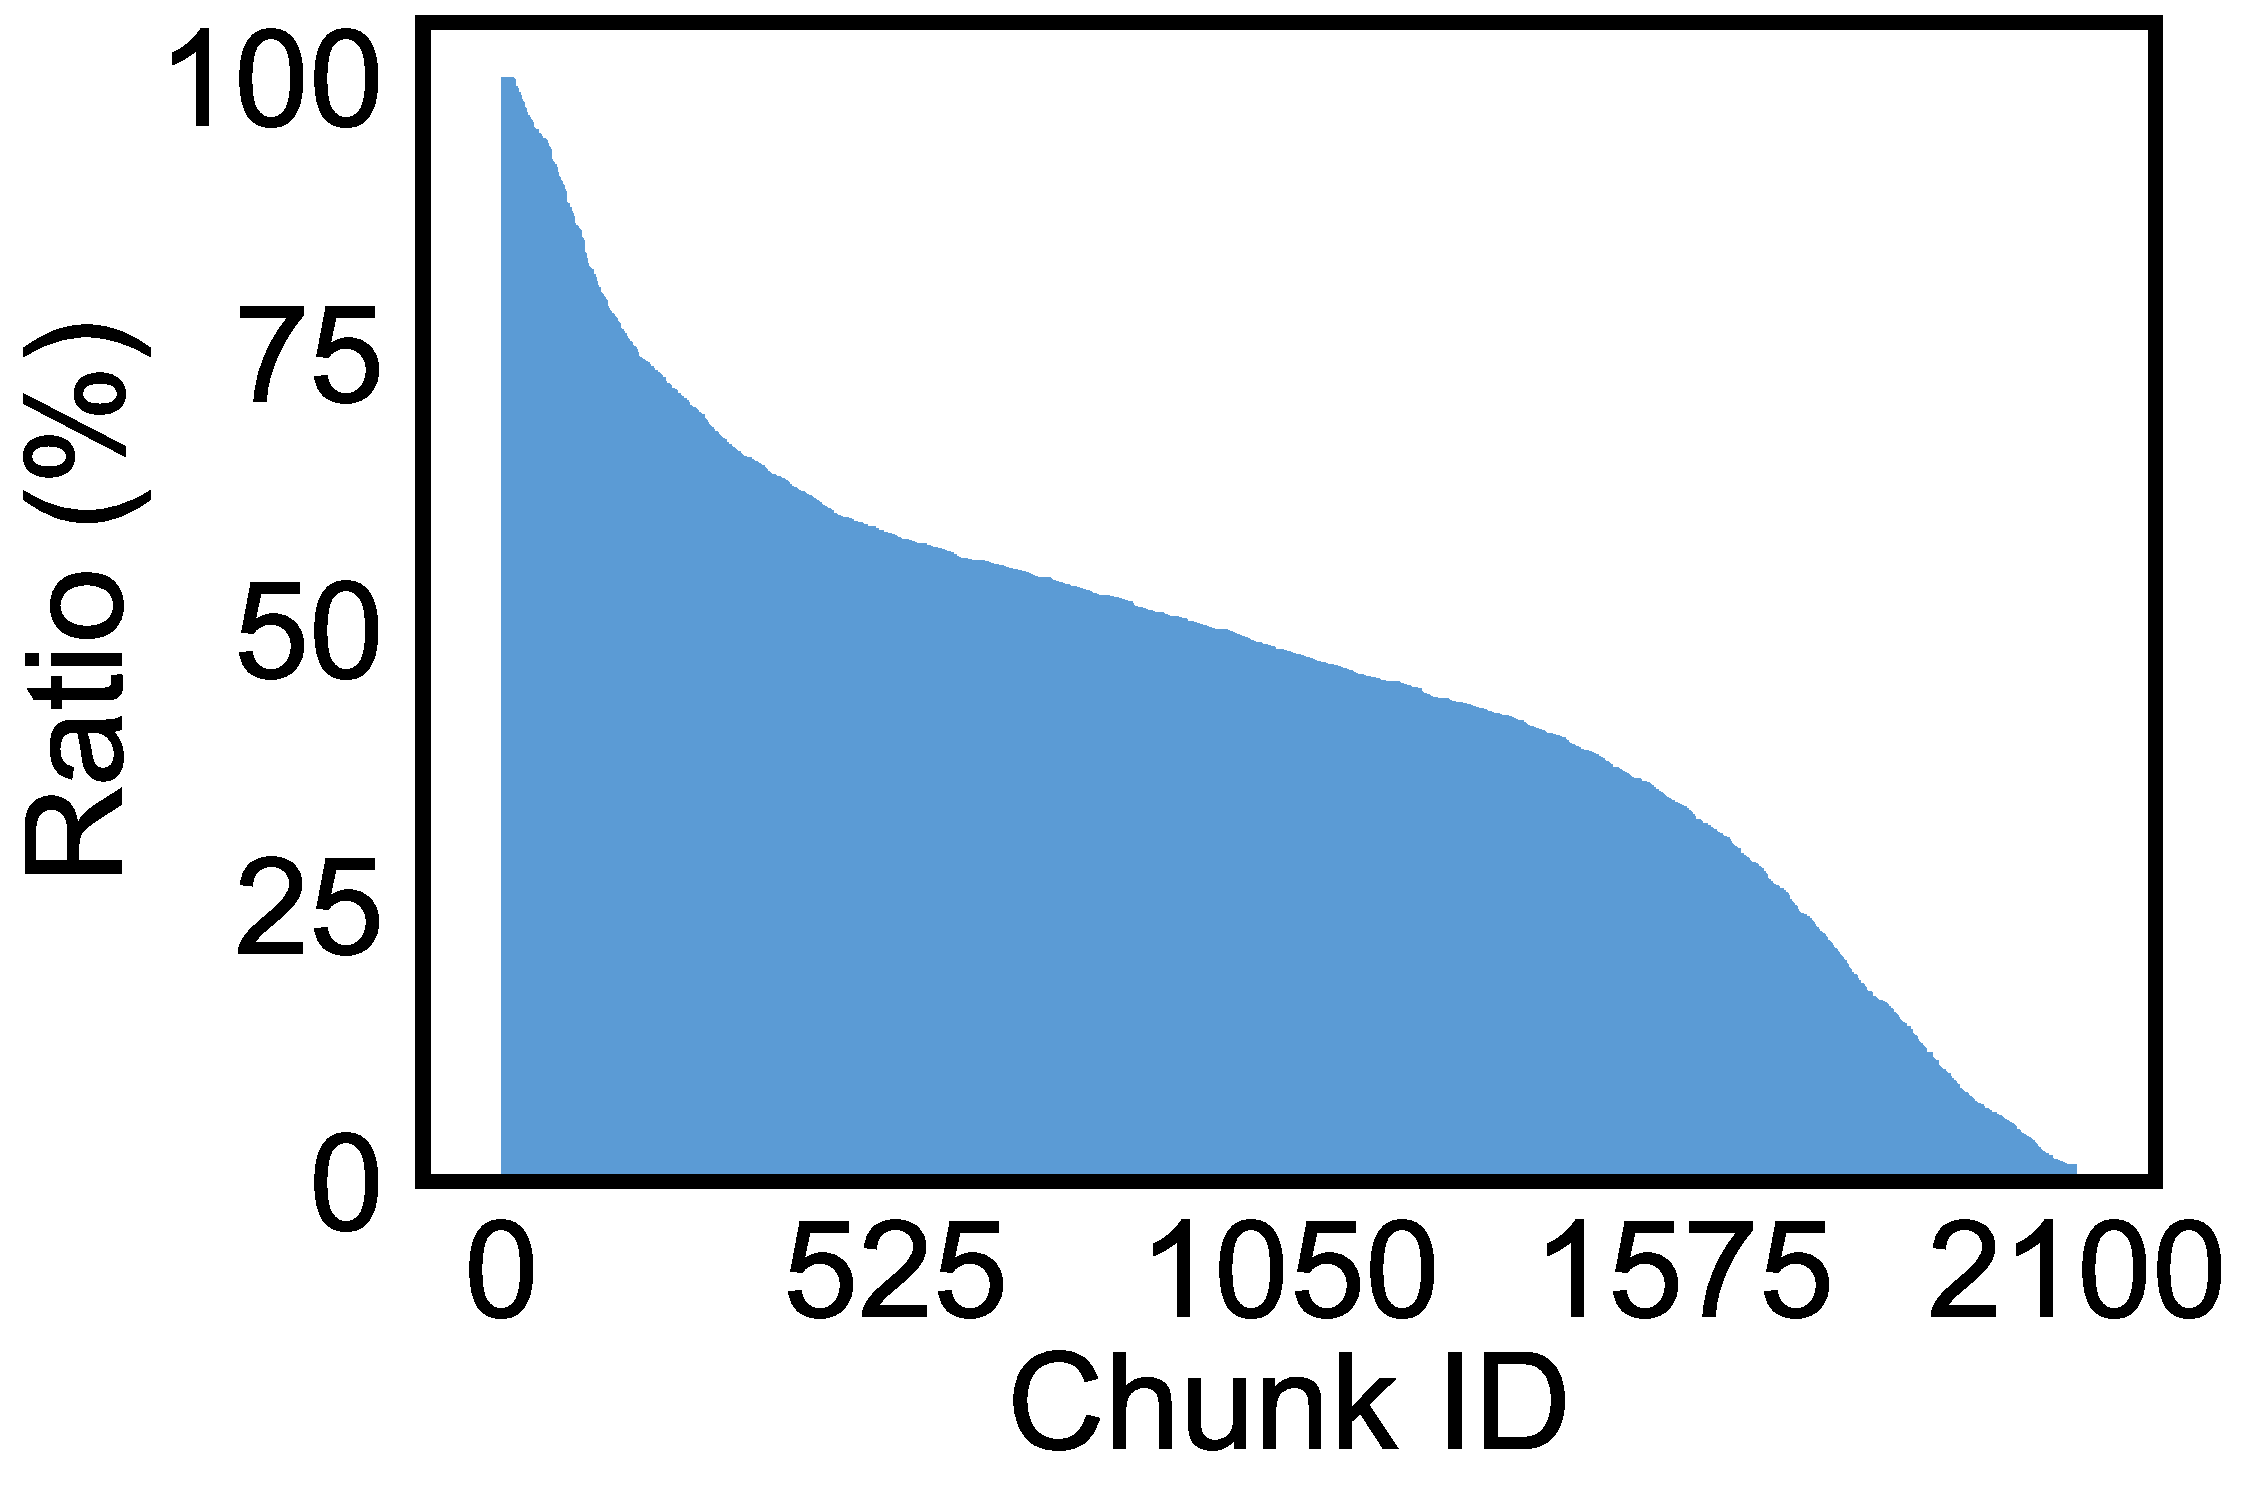
\includegraphics[width=1.5in, height=1in]{impratio_per_chunk.pdf}
		\label{fig:read_amplify}
	}
	\hspace{0.03in}
	\subfigure[]{
		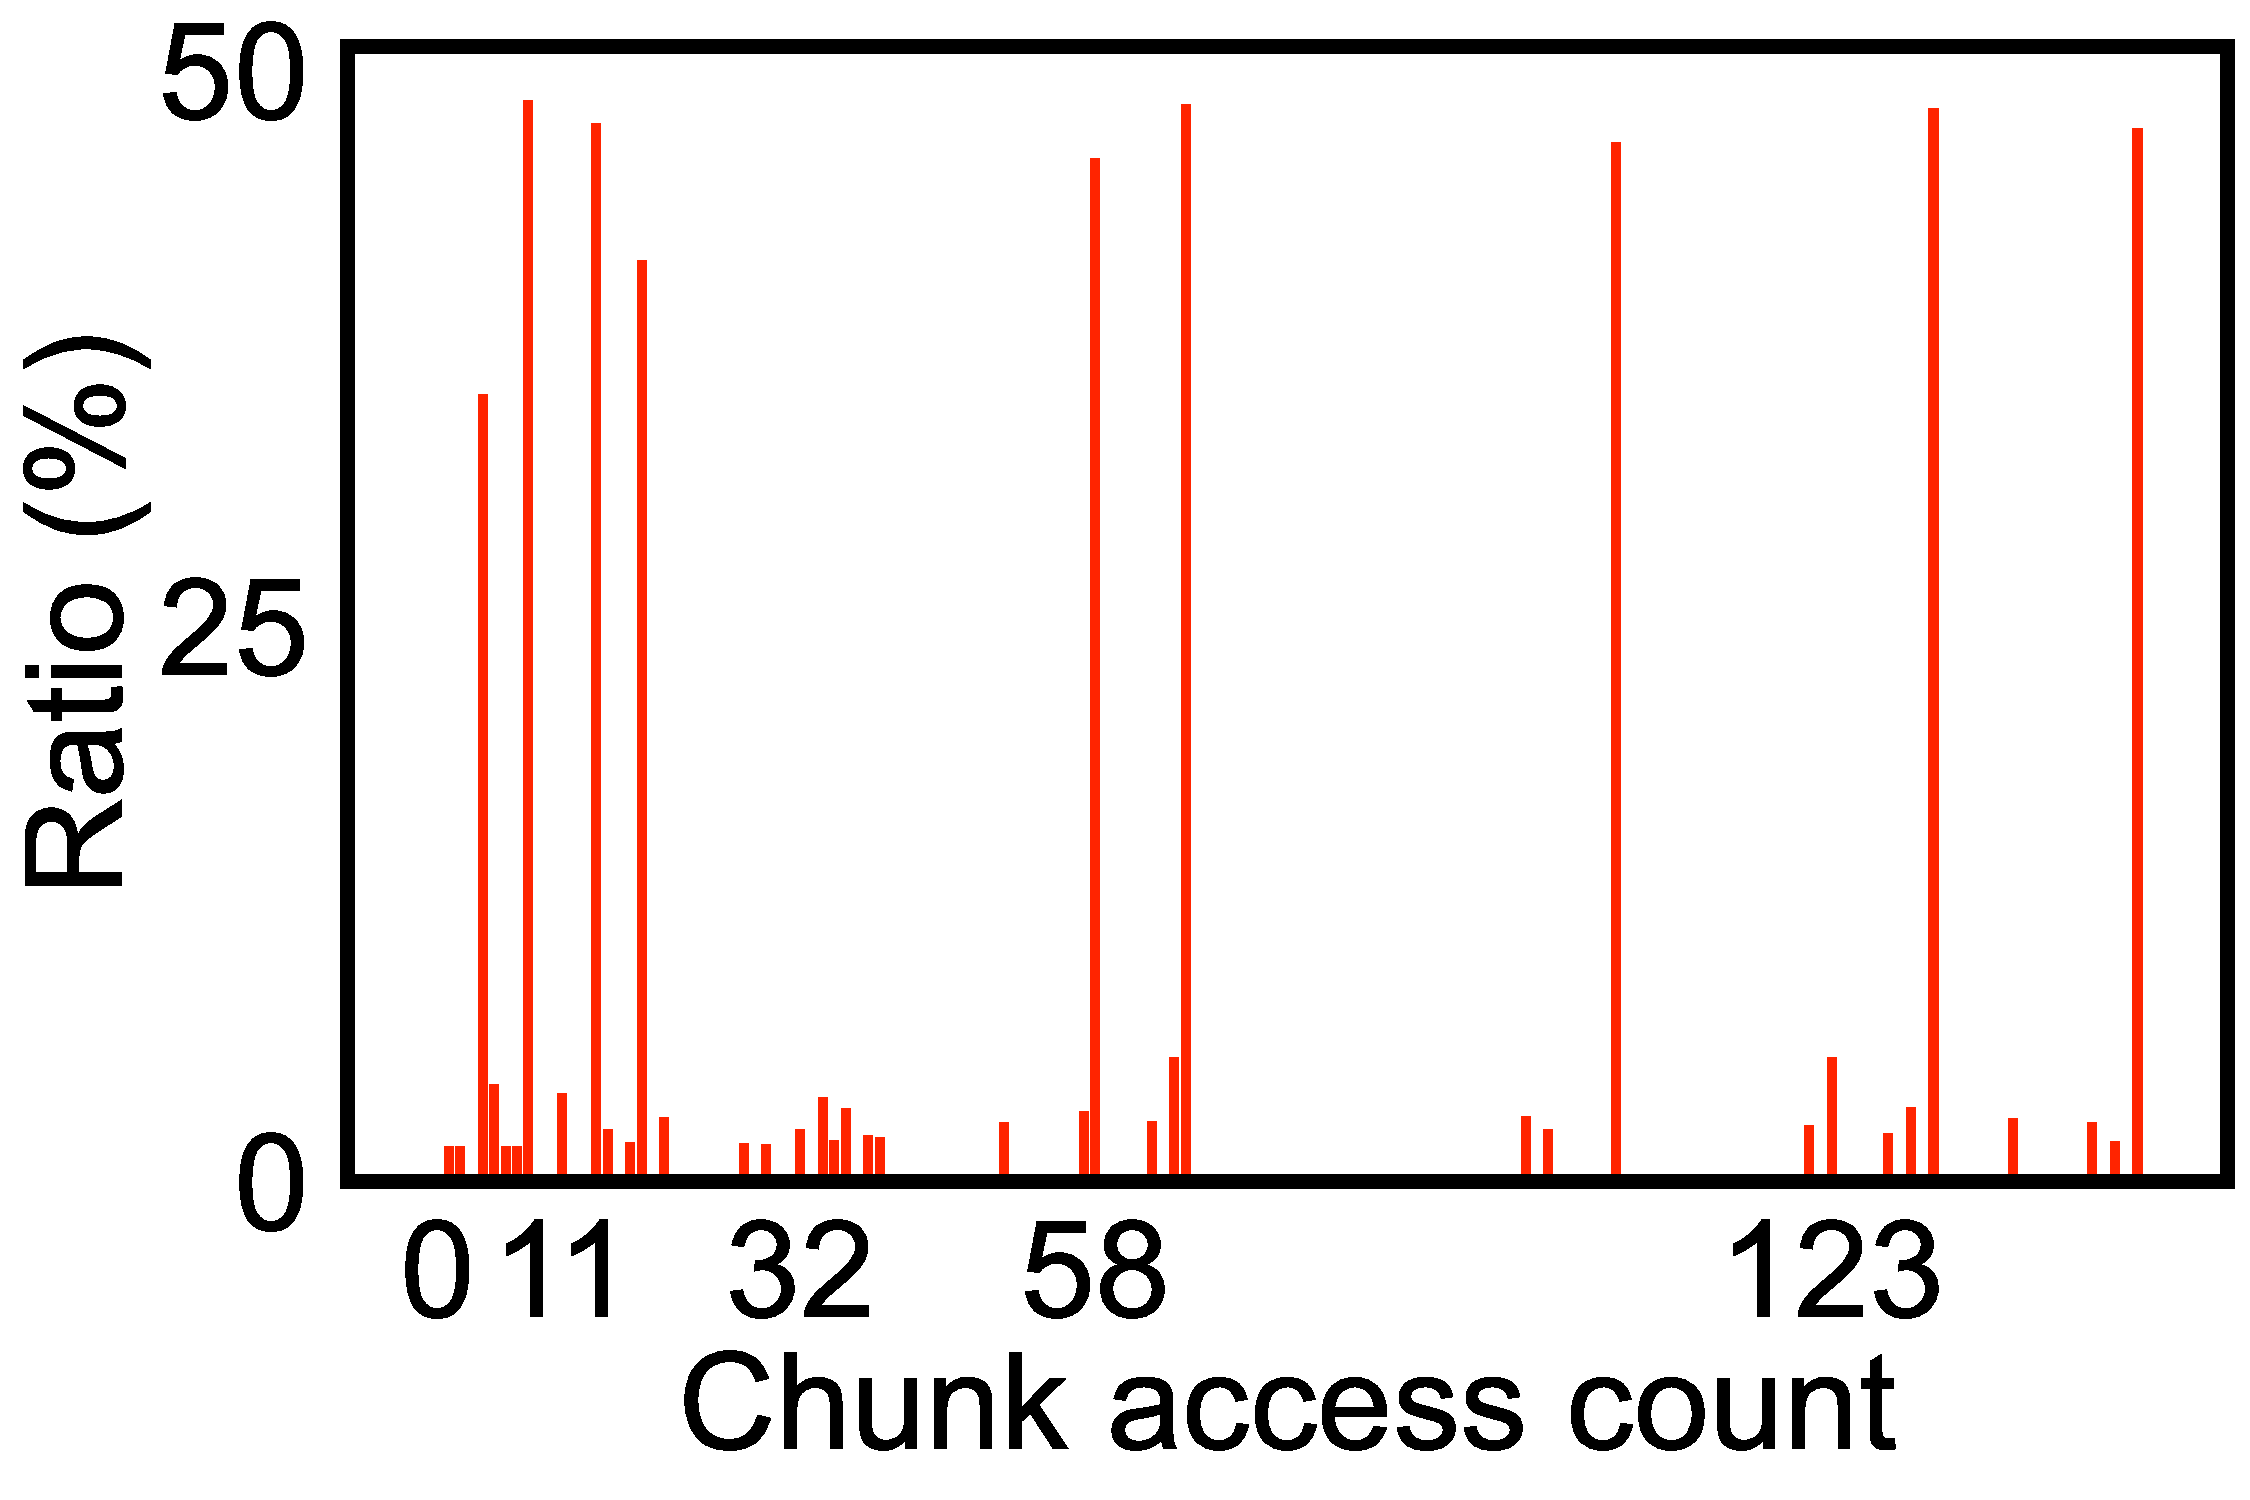
\includegraphics[width=1.5in, height=1in]{impratio_accesscount.pdf}
		\label{fig:imp_token_num}
	}
	\caption{
		(a) The ratio of important KVs within each chunk. 
		(b) Average ratio of important tokens in all chunks for a given chunk access frequency.}
	\label{fig:cha2}
\end{figure}

\noindent 
\zrdnew{
\textbf{Challenge 2: important tokens are unknown before prefetching.}
Existing methods determine the important KVs of each layer by computing the attention weights of the current layer. As a result, the distribution of important tokens for the next layer is not available during the current layer’s computation. This prevents prefetching of the next layer’s important KVs while the current layer is being processed, leaving I/O bandwidth underutilized. }

\zrdnew{A straightforward alternative is to randomly prefetch KVs for the next layer without considering their importance, 
but this approach suffers from low prefetch precision and loads numerous unimportant tokens’ KVs into GPU memory, wasting I/O bandwidth.}
To verify this, we measured the recall rate of randomly prefetching KVs across two models and datasets, xxx and xxx. As shown in Figure xxx, when KVs were pre-fetched randomly, the recall rate was only xxx. This approach leads to a large number of unimportant KVs being loaded into CPU memory, which are not used during inference, resulting in wasted I/O bandwidth and GPU memory.



\noindent 
%\textbf{Challenge 2: New approaches to store prefix KV and manage caches are required considering token's importance.}
\fvc{
\textbf{Challenge 3: The existing prefix KV storage and caching systems are suboptimal considering token's importance.}
}
Existing systems typically store and manage cache by grouping KV pairs from
several consecutive or all prefix tokens into
chunks~\cite{chunkattention-arxiv24, sglang-arxiv23, attentionstore-atc24,
hydragen-arxiv24}, which enhances the efficiency of disk reads and PCIe
transfers. 
% Each chuck contains multiple important and unimportant KVs. 
% When fetching important tokens' KVs, each request loads entire chunks into memory, including unimportant KVs. This leads to read 
% amplification and reduces effective read bandwidth. These unimportant KVs occupy additional cache space and decrease cache hit ratios.
% Moreover, directly managing chunks across both CPU and GPU cache spaces based on the traditional metrics like recency or frequency can degrade GPU cache hit ratios and increase the amount of data transferred over PCIe. 
% This is because they are oblivious of KV importance and do not consider the ratio of important KVs 
% in each chunk. Thus, they can place cold chunks with more important KVs in the CPU, while placing hot chunks with 
% fewer important KVs in the GPU. This misplacement reduces the hit ratio of important KVs in the GPU and requires 
% more important KVs to be transferred from the CPU to the GPU.
Each chunk contains a mix of important and unimportant KVs. When retrieving KVs for important tokens, entire chunks are loaded into memory, including the unimportant ones. This practice causes read amplification, diminishing effective bandwidth and filling cache with unnecessary data, which lowers cache hit ratios.

Furthermore, managing chunks in CPU and GPU caches based solely on traditional
metrics like recency or frequency can further reduce GPU cache hit ratios and
increase PCIe data transfers. This is because these metrics ignore the
importance of KVs and the proportion of important KVs in each chunk. As a
result, less critical chunks may occupy valuable GPU memory, while more critical
ones are relegated to the CPU memory. This misallocation decreases the GPU hit ratio
for important KVs and necessitates more data transfers between CPU and GPU memory.


We experimentally illustrate this challenge using OPT-6.7B on RTE. 
%We select the top 50\% most important KVs from each prefix for inference. 
% \wj{
We designate half of the prefix tokens as important and the remaining half as unimportant.
% }
Figure~\ref{fig:read_amplify} shows 
% the ratio of important KVs within each prefix KV chunk 
% that are selected for model inference. It shows 
that only 46\% of the KVs in the 
loaded chunks are important on average, leading to 2.2$\times$ read amplification. 
Figure~\ref{fig:imp_token_num} shows the ratio of important KVs for chunks with different access 
frequency. The hotness or coldness of a chunk is not related to the 
ratio of important KVs it contains. These observations 
% confirm the challenges mentioned above and 
underscore the need for new KV storage and cache management methods to reduce 
the loading of unimportant KVs from disk and improve cache hit ratios.
